\documentclass[UTF8,fontset=fandol,zihao=-4]{ctexart}
\usepackage[a4paper,margin=25mm]{geometry}
\usepackage{amsmath,amssymb,booktabs,array,graphicx,hyperref,xcolor}
\usepackage{caption,fancyhdr,placeins}
\hypersetup{colorlinks=true,linkcolor=blue,citecolor=blue,urlcolor=blue}
\setlength{\headheight}{15pt}
\setlength{\emergencystretch}{2em}
\pagestyle{fancy}\fancyhf{}\fancyhead[L]{ParallelBayes：执行成本与推断误差}\fancyfoot[C]{\thepage}
\newcommand{\E}{\mathbb{E}}
\newcommand{\R}{\mathbb{R}}
\title{时间并行 MCMC 的执行成本与推断误差：基于 ParallelBayes 的比较研究}
\author{中文研究稿：作者与单位待定}
\date{2026 年 10 月 12 日 · v5}

\newcommand{\ind}{\mathbf{1}}

% Generated from a verified scalar bundle; do not edit numbers by hand.
\newcommand{\PBCompactValid}{3741}
\newcommand{\PBCompactNumerical}{42}
\newcommand{\PBCompactUnclassified}{105}
\newcommand{\PBCompactFunctionRows}{14981}
\newcommand{\PBCompactHighRhat}{5000}
\newcommand{\PBCompactUndefinedRhat}{1290}
\newcommand{\PBCPURWMMin}{0.424}
\newcommand{\PBCPURWMMax}{1.178}
\newcommand{\PBCPURWMAbove}{7}
\newcommand{\PBCUDARWMMin}{0.953}
\newcommand{\PBCUDARWMMax}{1.659}
\newcommand{\PBCUDARWMAbove}{14}
\newcommand{\PBCPUMALAMin}{0.116}
\newcommand{\PBCPUMALAMax}{0.394}
\newcommand{\PBCPUMALAAbove}{0}
\newcommand{\PBCUDAMALAMin}{0.234}
\newcommand{\PBCUDAMALAMax}{0.408}
\newcommand{\PBCUDAMALAAbove}{0}

% Generated by review3_numerics.py; saved evidence only.
\newcommand{\PBIIDLTwoStates}{4128768}
\newcommand{\PBIIDLTwoHits}{0.0064635}
\newcommand{\PBIIDLTwoZero}{99.356}
\newcommand{\PBIIDWOneStates}{4423680}
\newcommand{\PBIIDWOneHits}{0.000210886}
\newcommand{\PBIIDWOneZero}{99.979}

\begin{document}
\maketitle
\begin{abstract}
时间并行马尔可夫链蒙特卡罗（MCMC）先猜测一段采样轨迹，再同时修正多个时间位置，尝试缩短单条链的计算时间。我们用带R接口的ParallelBayes比较Online Picard随机游走Metropolis与窗口quasi-DEER MALA，并通过预先保存的随机数和独立顺序实现检查状态及接受事件。九个目标、两档链长和CPU/CUDA的3888次四链拟合中，3741次满足各自输出标准；通过检查的MH主任务及缓存回放共约5445万次转移，接受事件零失配。包含进程启动、采样和诊断的批量推断时间下，Picard的顺序/并行耗时比在CPU上为0.42--1.18，在CUDA上为0.95--1.66；quasi-DEER在全部36组比较中更慢。水井回归中，CPU顺序RWM用约4.9秒完成一次拟合；NUTS用约2.4倍时间，将截距的参考平方误差降至约七分之一。窗口对照和分段计时说明，重复求值与工作流开销共同影响收益。全拒绝轨迹的执行加速、均衡初值维持的双峰权重，以及稀有事件的极小绝对误差，进一步说明执行时间需要与后验函数误差和探索诊断一起评价。
\end{abstract}
\noindent\textbf{关键词：}时间并行MCMC；Metropolis--Hastings；计算成本；轨迹核验；GPU；R

\section{引言}
马尔可夫链蒙特卡罗（Markov chain Monte Carlo，MCMC）是贝叶斯计算的重要工具。常规采样按时间顺序更新状态，下一步依赖当前结果。多核CPU与GPU则擅长同时完成许多计算：同时运行多条链可以增加吞吐，如何利用这些资源缩短一条指定轨迹的计算时间，仍是另一项计算问题。

时间并行从确定性递推的角度处理这种依赖。把初值和采样所需随机数固定后，整条链就是一组递推方程的解。执行器可以先猜测路径，在各时间位置同时计算更新，再反复修正猜测。Newton类方法用近似导数求解整段路径，Online Picard则重建接受增量，并逐步确认匹配的前缀\cite{zoltowski,grazzi}。两条路线都增加了重复求值和同步工作，实际收益取决于并行吞吐能否抵消这些开销。

我们区分两个研究问题。\textbf{第一，同一个转移核能否被更快地执行？}比较固定初值、核参数和实际随机数组的顺序与时间并行计算。\textbf{第二，计算时间换来了多少推断信息？}比较合理配置下不同核的后验函数误差，同时检查初始化和探索情况。前者控制轨迹的统计内容，后者还受到核与调参的影响。

已有compareMCMCs、PPL Bench和posteriordb支持跨引擎运行、基准设计或参考目标\cite{comparemcmcs,pplbench,posteriordb}；ParallelMCMC.jl提供时间并行MALA接口，BayesForge连接R建模与JAX推断\cite{parallelmcmc,bayesforge}。ParallelBayes将目标、转移核和执行方式分开，并保存逐步核验所需输入。我们据此完成三项工作：在同一随机数组上比较路径和接受事件；用明确的计时边界比较执行成本；通过函数误差、拒绝状态和模式探索解释速度比的统计含义。

研究的主要发现是，所测Picard实现的批量成本收益较小且依赖设备，quasi-DEER的额外工作未被抵消。核选择可以显著改变误差，但这种改善也依赖目标与配置。下文先介绍算法和核验，再说明软件、实验设计和结果；实现历史及完整逐函数结果分别见补充材料A、B。

\section{时间并行方法与路径核验}
\subsection{目标坐标与转移核}
采样器在无约束坐标中工作，因此不同实现首先需要计算相同目标。若$T$是相应自由坐标间的可微一一变换、原参数$\theta=T(q)$，计算密度为
\begin{equation}
\ell(q)=\log p(y,T(q))+\log|\det J_T(q)|.
\end{equation}
我们核对同坐标下的密度差$\ell(q)-\ell(q_0)$、梯度和参数变换；这也允许实现省略不同的参数无关常数。

随机游走Metropolis（random-walk Metropolis，RWM）使用$q'=q+sz$，$z\sim N(0,I_d)$，接受对数比为$\ell(q')-\ell(q)$。Metropolis调整Langevin算法（Metropolis-adjusted Langevin algorithm，MALA）使用
\begin{align}
q'&=q+h\nabla\ell(q)+\sqrt{2h}\,z,\\
a(q,q')&=\ell(q')-\ell(q)-\frac{\|q-q'-h\nabla\ell(q')\|^2-\|q'-q-h\nabla\ell(q)\|^2}{4h}.
\end{align}
对独立$u\in(0,1)$，当$\log u<a(q,q')$时接受，否则保留$q$。$h$是漂移步长，提议噪声标准差为$\sqrt{2h}$。拒绝产生的自环也计为一次转移。

\subsection{把随机性与执行顺序分开}
核验的关键是先生成并保存提议噪声$z_t$与接受判断所需$u_t$。这些数组一旦固定，每一步成为确定映射$F_t$，顺序路径满足
\begin{equation}\label{eq:recurrence}
q_t^\star=F_t(q_{t-1}^\star),\quad t=1,\ldots,W.
\end{equation}
顺序执行逐步计算这个递推，时间执行器按另一种计算顺序求解它。我们使用单独编写的NumPy密度、解析梯度和显式循环作为参考，它不调用待测JAX或torch转移函数。整数种子相同不足以实现这种比较，运行间传递的是已保存的实际数组。

\subsection{quasi-DEER：仿射修正整段路径}
quasi-DEER对整段路径作近似Newton修正。在第$k$轮路径上计算映射和近似矩阵$B_t^{(k)}$，再求解
\begin{equation}\label{eq:deer}
q_t^{(k+1)}=F_t(q_{t-1}^{(k)})+
B_t^{(k)}\{q_{t-1}^{(k+1)}-q_{t-1}^{(k)}\}.
\end{equation}
给定旧路径后，右侧是新前驱的仿射函数。仿射映射的复合满足结合律，因此这些更新可通过树形扫描同时求解。

这种因果递推具有一个有限轮性质：在精确算术、映射有定义、矩阵有限且仿射递推精确求解时，第$k$轮至少恢复前$k$个状态，长度$W$的窗口至多需要$W$轮\cite{gonzalez,zoltowski}。固定初值使第一步正确；当前若前$k$步已经正确，下一轮保留该前缀，并使第$k+1$步的修正项为零。矩阵近似影响推进速度；最坏每轮仍对$W$个位置求值，映射总工作量可达顺序递推的$W$倍。实际浮点程序另采用残差停止与外部路径检查。

硬MH判断的分支发生跳变，因此我们通过直通构造（straight-through construction）生成代理Jacobian。令$b=\ind\{\log u<a\}$、$\operatorname{sg}$表示停止梯度，门控公式为
\begin{equation}
g=b+\sigma(a-\log u)-\operatorname{sg}\{\sigma(a-\log u)\}.
\end{equation}
前向使用硬接受结果，求导使用平滑代理。对每链、每个时间位置固定一个Rademacher向量$v_t$，以Jacobian--向量积（JVP）构成Hutchinson型对角近似：
\begin{equation}
B_t^{(k)}=\operatorname{Diag}\!\left[\operatorname{clip}\{v_t\odot(J_{\mathrm{proxy},t}^{(k)}v_t),-1,1\}\right].
\end{equation}
探针在窗口各轮间复用，截断仅作用于导数近似。本文实现使用非重叠窗口、重复窗口起点的初猜和硬残差停止；门控与上游实现的版本差异及数值处理见补充材料A。

\subsection{Online Picard：重建并确认前缀}
Online Picard先用上一轮猜测的前驱计算接受增量，累加出新路径，再检查这些接受决策在新前驱上是否仍成立。以已确认起点$q_L$为锚，
\begin{align}
D_t^{(k)}&=sz_t\ind\{\log u_t<\ell(q_{t-1}^{(k)}+sz_t)-\ell(q_{t-1}^{(k)})\},\\
q_t^{(k+1)}&=q_L+\sum_{i=L+1}^{t}D_i^{(k)}.
\end{align}
固定噪声后，接受事件匹配便确定相同增量。由起点向后归纳，连续匹配的前缀满足原递推\cite{grazzi}。例如“匹配、匹配、不匹配、匹配”只允许确认前两个位置（图\ref{fig:prefix}）。torch批量实现取各链最短确认长度共同推进，因此批内推进最慢的一条链决定进度。
\begin{figure}[htbp]\centering
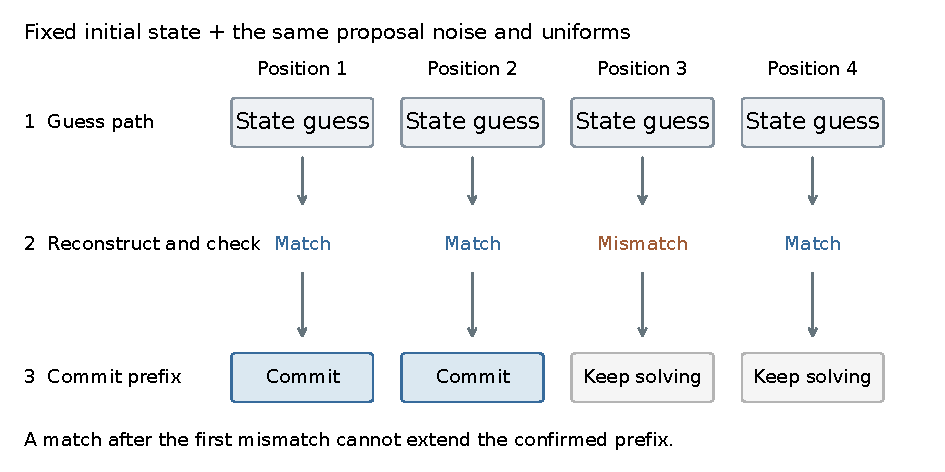
\includegraphics[width=\linewidth]{../../figures/manuscript-v5/trajectory-schematic.pdf}
\caption{Online Picard的一次路径检查。四个位置依次为匹配、匹配、不匹配、匹配；只能提交起点之后连续匹配的前两个位置。第四个位置单独匹配，其前驱仍需修正。图为概念示意。}\label{fig:prefix}
\end{figure}

\subsection{内部停止和外部核验}
我们分别检查局部递推与整条参考路径。quasi-DEER的内部停止条件为
\begin{equation}
r=\max_{t,j}\frac{|q_{t,j}-F_t(q_{t-1})_j|}{\mathrm{atol}+\mathrm{rtol}|F_t(q_{t-1})_j|}\le1.
\end{equation}
外部核验要求接受事件零失配，每链最大路径差不超过
\begin{equation}\label{eq:tolerance}
\tau=100[\mathrm{atol}+\mathrm{rtol}\max(1,\max|q|)],\qquad
\mathrm{atol}=\mathrm{rtol}=10^{-10}.
\end{equation}
该工程标准容许不同累加次序造成的浮点偏差，阈值随整条路径的状态幅度放大。我们同时报告路径差与$\tau$之比。局部残差与全局路径差分别衡量，两项检查并行使用。

迭代耗尽、非有限值或外部检查未通过时，保存失败轨迹及成本，输出不计入正式推断样本。NUTS使用自身随机流和预热，检查输出完整性、有限性及独立统计诊断，采用另一套运行契约。正文中的“通过核验”表示满足对应数值输出标准，探索质量由后续诊断和函数误差评估。

\section{软件与R使用流程}
\subsection{目标、核和执行方式分开组织}
R负责组织模型、配置和结果，数值循环由编译密度接口或Python后端执行。Stan/BridgeStan提供C++密度与导数\cite{stan,bridgestan}；原生JAX目标支持JIT与批处理，并接入BlackJAX\cite{blackjax}；原生torch目标支持Windows CPU/CUDA，时间执行器目前由Python逐轮控制。CPU Pyro NUTS\cite{pyro}通过独立研究命令行工具运行。支持范围见表\ref{tab:capabilities}。
\begin{table}[htbp]\centering\small
\begin{tabular}{p{.29\linewidth}p{.15\linewidth}p{.31\linewidth}p{.14\linewidth}}\toprule
目标入口 & 顺序RWM/MALA & Picard RWM / quasi-DEER MALA & NUTS\\\midrule
Stan/BridgeStan，Mac CPU & $\checkmark$ & --- & ---\\
明确JAX目标，CPU & $\checkmark$ & $\checkmark$ & BlackJAX\\
明确torch目标，Windows CPU & $\checkmark$ & $\checkmark$ & Pyro研究CLI\\
明确torch目标，Windows CUDA & $\checkmark$ & $\checkmark$ & ---\\\bottomrule
\end{tabular}
\caption{当前目标入口与方法支持范围。时间执行器仅支持表列对应核；Pyro四链基线使用独立研究CLI。}\label{tab:capabilities}
\end{table}

用户用\texttt{pb\_model()}建立内置或Stan目标，\texttt{pb\_capabilities()}查询包接口组合，\texttt{pb\_sample()}返回样本及运行记录。\texttt{pb\_benchmark()}运行给定配置列表，结果可转入\texttt{posterior}进行分析\cite{posterior}。完整实验的输入清单、恢复和证据归档由研究CLI负责。自定义模型通过公开Python \texttt{Model}接口提供密度、梯度和独立NumPy参考，再由R调用；完整Poisson扩展示例见补充材料A。

\subsection{一个可运行的调用例子}
以下示例使用二维标准高斯与顺序/Picard RWM。启动R前选择Python环境并安装R包；完整脚本\texttt{examples/paper-api-v5.R}接受一个新输出目录，保存两份拟合及诊断。
\begingroup\small\begin{verbatim}
library(parallelbayes)
model <- pb_model("gaussian", dimension = 2L, backend = "torch")
stopifnot(pb_validate(model)$passed)
configs <- lapply(c("sequential", "online_picard"), function(executor)
  list(kernel = "rwm", executor = executor, device = "cpu",
       draws = 8192L, chains = 4L, step_size = 0.8, window = 16L,
       max_iter = 8704L, seed = 2026L, audit = TRUE))
fits <- pb_benchmark(model, configs)
stopifnot(identical(fits[[1]]$record$tape_sha256,
                    fits[[2]]$record$tape_sha256),
          identical(fits[[1]]$record$accept, fits[[2]]$record$accept))
posterior::summarise_draws(fits[[2]]$draws)
\end{verbatim}\endgroup

本例在安装版R包与Mac torch CPU上实际运行。两种执行均通过独立参考检查，最大路径差为$1.1\times10^{-14}$，两参数诊断见表\ref{tab:r-example}。这是单个技术示例，独立于正式实验的24次重复。
\begin{table}[htbp]\centering\small
\begin{tabular}{lrrrrr}\toprule
参数 & 均值 & 标准差 & $\hat R$ & bulk ESS & tail ESS\\\midrule
$q_1$ & 0.00693 & 1.014 & 1.00166 & 2129 & 3169\\
$q_2$ & -0.00311 & 1.003 & 1.00042 & 2823 & 4427\\\bottomrule
\end{tabular}
\caption{公开R接口示例的实际输出（Picard，四链各8192步）。ESS为有效样本量（effective sample size）；bulk和tail分别描述主体与尾部。}\label{tab:r-example}
\end{table}

R启动费用另以既有Poisson输入直接测量。32个新进程、64次技术调用中，普通模式首次结果与诊断可用延迟的组中位数为1.3--2.1秒，同会话第二次完整调用为0.014--0.340秒。重复调用复用环境与准备工作；本测量与下文Windows主实验的批量边界分开，完整观测及分段计时见补充材料A。

\section{实验设计}
\subsection{目标库与比较配置}
主实验在Windows 11、Ryzen 7 9800X3D与RTX 5080上运行，所有数值使用float64。九个目标区分维度、坐标表示、观测量和模式结构（表\ref{tab:targets}）。G2和A1先作完整协方差白化，采样坐标为标准高斯；H1/H2则把同一漏斗后验写成两种坐标。原尺度函数经参数映射对应。
\begin{table}[htbp]\centering\small
\begin{tabular}{p{.24\linewidth}rp{.30\linewidth}p{.29\linewidth}}\toprule
目标 & 维数 & 定义/计算坐标 & 选择目的\\\midrule
G1 独立高斯 & 8 & $N(0,I)$ & 简单可解析对照\\
G2 相关高斯 & 64 & 原协方差条件数100；完整白化 & 白化后的维度效应\\
A1 潜在AR(1) & 64 & $\rho=0.9$，噪声方差1；高斯后验白化 & 结构化目标与解析核对\\
L1 Logistic回归 & 8 & 256观测；正态系数先验 & 低成本非高斯似然\\
L2 Logistic回归 & 8 & 4096观测；正态系数先验 & 数据量与稀有事件\\
H1 中心化漏斗 & 9 & $v\sim N(0,9)$，$x\mid v\sim N(0,e^vI_8)$ & 尺度耦合与数值压力\\
H2 非中心化漏斗 & 9 & $x=e^{v/2}z$，$z\sim N(0,I_8)$ & 参数化对照\\
M1 双峰混合 & 8 & 等权$N(\pm5e_1,I)$ & 初始化与模式探索\\
W1 水井回归 & 2 & 3020观测；截距/距离系数平坦先验 & 真实数据推断案例\\\bottomrule
\end{tabular}
\caption{主实验的九个目标。Logistic系数先验标准差为2.5；数据与完整公式、仿射坐标来源见补充材料A。}\label{tab:targets}
\end{table}

每目标24份独立四链输入，每链分别保留1024或4096步。RWM与MALA各有CPU/CUDA的顺序和时间执行组合，另有CPU四进程NUTS，共九种工作流（表\ref{tab:workflows}）。主实验因此包含$9\times9\times2\times24=3888$次四链拟合。同核执行共享初值、核参数和实际随机数组；配对速度比在同后端、同设备内计算。NUTS与MH的误差--成本比较属于不同完整工作流的比较。
\begin{table}[htbp]\centering\small
\begin{tabular}{lclc}\toprule
核 & 设备 & 执行方式 & 工作流数\\\midrule
RWM & CPU、CUDA & 顺序、Online Picard & 4\\
MALA & CPU、CUDA & 顺序、窗口quasi-DEER & 4\\
NUTS & CPU & Pyro四进程，每进程一条链 & 1\\\bottomrule
\end{tabular}
\caption{九种正式工作流。NUTS为无转向采样器（No-U-Turn Sampler），采用独立随机流与自适应预热。}\label{tab:workflows}
\end{table}

\subsection{调参、初始化和预算}
我们先在独立开发输入上选择MH配置：每目标、每核六个候选，每候选两份四链输入，在两份都满足数值标准的候选中最大化平均标准化跳跃平方距离（ESJD/d）。216次开发运行中212次完成，4次失败。该准则衡量移动距离，正式函数误差随后独立评价。回归目标使用众数与信息矩阵形成仿射坐标；最终步长及开发成本见补充材料A。

表\ref{tab:settings}列出主实验设置。窗口32用于固定一个受控的执行配置，既有机制对照另考察窗口变化；它是设计选择，并未经全目标窗口优化。完整资源保护与运行顺序见补充材料A。
\begin{table}[htbp]\centering\small
\begin{tabular}{lp{.65\linewidth}}\toprule
项目 & 设置\\\midrule
初值 & 采样坐标$N(0,4I)$；M1首坐标按两负两正放置\\
保留与丢弃 & 每链保留1024/4096步；MH丢弃512步\\
时间窗口与迭代 & 窗口32；quasi-DEER每窗口最多2048轮，Picard最多$N+512$轮\\
NUTS适应 & 每链预热1024步；目标接受率0.8；最大树深8；对角质量矩阵\\
CPU执行 & MH使用4个torch线程；NUTS四进程，各1个torch线程\\\bottomrule
\end{tabular}
\caption{主实验的固定配置。两档预算是已测点，研究没有在二者之间插值得到达标时间。}\label{tab:settings}
\end{table}

\subsection{函数误差、参考与不确定性}
对每个预先规定的函数$f$，每份四链输入给出合并估计$\widehat\mu_{a,f}^{(r)}(N)$。令$\mathcal V_{a,f,N}$为满足数值输出标准且函数估计有限的重复集合，计算
\begin{equation}\label{eq:error}
\widehat E^{\,\mathrm{valid}}_{a,f}(N)=
\frac1{|\mathcal V_{a,f,N}|}\sum_{r\in\mathcal V_{a,f,N}}
(\widehat\mu_{a,f}^{(r)}(N)-\mu_f^\star)^2.
\end{equation}
有解析期望时，它估计成功条件下的均方误差（MSE）；使用有限参考时，称相对参考值的平方误差。比较两方法时另取共同有效集合，失败率使用全部24次计划重复。诊断不良的有效轨迹仍进入上述统计。
\begin{table}[htbp]\centering\small
\begin{tabular}{>{\raggedright\arraybackslash}p{.15\linewidth}>{\raggedright\arraybackslash}p{.40\linewidth}>{\raggedright\arraybackslash}p{.33\linewidth}}\toprule
目标（函数数） & 原尺度函数 & 期望/参考\\\midrule
G1/G2/A1（各3） & $z,\ z^2,\ \ind(z>1)$，$z=(\theta_1-m_1)/\sqrt{\Sigma_{11}}$ & $0,1,1-\Phi(1)$\\
L1/L2（各4） & $\theta_1,\theta_2,\sigma(\theta_1),\ind(\theta_1>0)$ & 独立NUTS有限参考；L2事件另有重要性参考\\
H1/H2（各4） & $v/3,\tanh(v/3),\ind(x_1>0),\cos(x_1e^{-v/2})$ & $0,0,1/2,e^{-1/2}$\\
M1（4） & $\theta_1/\sqrt{1+\delta^2},\ind(\theta_1>0),\theta_2,\theta_2^2$ & $0,1/2,0,1$；$\delta$为模式位置绝对值\\
W1（7） & $\alpha,\beta,\alpha^2,\beta^2,\sigma(\alpha),\sigma(\alpha+\beta),\ind(\beta>0)$ & 区间数值包络及独立有限参考；非解析真值\\\bottomrule
\end{tabular}
\caption{九目标共36个函数；W1两项预测概率对应0米和100米。最终配置见补充材料第1节，逐函数参考与精度见第2节。历史$s_f=1$口径保留，不用正式样本方差重新归一化。}
\label{tab:functions}
\end{table}

函数中的标准化如$z$、$v/3$直接包含在定义里，其余函数保持原单位。原协议的额外尺度均为1，式\eqref{eq:error}省去这一因子；各函数的误差大小仍需按其实际含义解释。

参考值按证据来源使用。高斯、漏斗和混合目标有解析期望；Logistic连续函数使用独立长链NUTS参考；L2符号事件新增两套独立重要性参考及近似MCSE。W1另通过球算术、求积余项与尾界得到数值区间。原参考及其不确定性继续用于历史图表，新增区间与重要性参考分别检验其敏感性（补充材料A）。

我们用\texttt{posterior}计算秩正态化/折叠$\hat R$、主体和尾部ESS\cite{vehtari,posterior}；常量链等退化结果保留不可判定。独立统计单位是一份随机输入上的完整四链拟合，链、配对执行、设备副本和缓存重放均不增加$n$。误差和耗时采用9999次BCa（偏差校正与加速）自助法，整次四链拟合整体重抽样，少于20份共同有效重复时不报区间。所示95\%区间逐点且条件于有效集合，未作同时覆盖或参考误差传播。

\subsection{三种计时边界}
我们区分准备后的执行、普通批量推断和包含核验的研究运行（表\ref{tab:cost-scope}）。CUDA边界显式同步；所有时间都是对应工作流的实际墙钟时间。普通批量时间包含其进程启动和R诊断，却不含最外层R前端、环境安装、独立开发调参或全局上传。上一节的R使用测量单独覆盖前端边界。
\begin{table}[htbp]\centering\small
\begin{tabular}{p{.23\linewidth}p{.44\linewidth}p{.24\linewidth}}\toprule
口径 & 包含的主要工作 & 回答的问题\\\midrule
准备后的内核 & 模型和设备已准备后的指定执行器调用 & 执行本身耗时多少？\\
普通批量推断 & 进程启动、目标准备、适应/丢弃、采样、转换、输出与R诊断 & 一次批量结果需等多久？\\
含核验研究运行 & 普通批量推断，加独立顺序参考与证据检查/归档 & 完整研究检查付出多少？\\\bottomrule
\end{tabular}
\caption{三种计时口径。后两项为嵌套边界，分别报告，不能相加。}\label{tab:cost-scope}
\end{table}

缓存仅对G1/G2/L2/W1安排256份探测，各重复调用4次。它们只提供执行成本，不增加正式后验样本数。历史Mac与Windows探索实验及其不同计时/预算设置见补充材料A；本文主结果以这次3888项实验为主。

\section{结果}
\subsection{配对执行满足路径标准，漏斗揭示标准的边界}
通过外部路径检查的MH输出逐步恢复了指定参考递推。3414次有效MH主拟合与1024次缓存调用共检查约5445万次转移，接受事件失配为零；主任务路径差与式\eqref{eq:tolerance}阈值的比值最大为0.884。另有327次NUTS满足其自身输出标准，3741项有效、42项轨迹检查失败和105项未分类运行失败合计为3888项。

42项轨迹检查失败全部来自中心化漏斗H1，其中40项为quasi-DEER，2项为顺序MALA；前者均已达到内部残差阈值。既有候选与独立NumPy路径的四个测试函数逐点差最大为$3.3\times10^{-3}$，四链合并均值差最大为$3.1\times10^{-7}$，接受事件一致。路径差可受复杂几何和累加次序放大，而均值差受持续时间及抵消影响；原42项继续按协议排除，函数检查描述另见补充材料A。

小型模拟校准（simulation-based calibration，SBC）与解析区间采用同一批64数据集。解析90\%区间覆盖54例，MALA覆盖同样数量但有4例配对覆盖分歧；逐数据集检查因此比仅比较总体比例更有信息，详见补充材料A及测试量选择的讨论\cite{modrak}。

\subsection{Picard收益依赖设备，quasi-DEER额外工作占优}
按普通批量推断时间计，Picard在CUDA上的多数目标--预算组具有加速点估计，在CPU上收益较小且不一致（图\ref{fig:compact-cost}）。速度比定义为顺序时间除以时间并行时间，大于1表示并行较快。CUDA的18组中14组点估计超过1，范围0.95--1.66；CPU中7组超过1，范围0.42--1.18。quasi-DEER的CPU范围0.12--0.39、CUDA范围0.23--0.41，即比顺序MALA多花约2.4--8.6倍时间。区间显示每组的不确定性，点估计超过1的组数不等同于证实加速的组数。
\begin{figure}[htbp]\centering
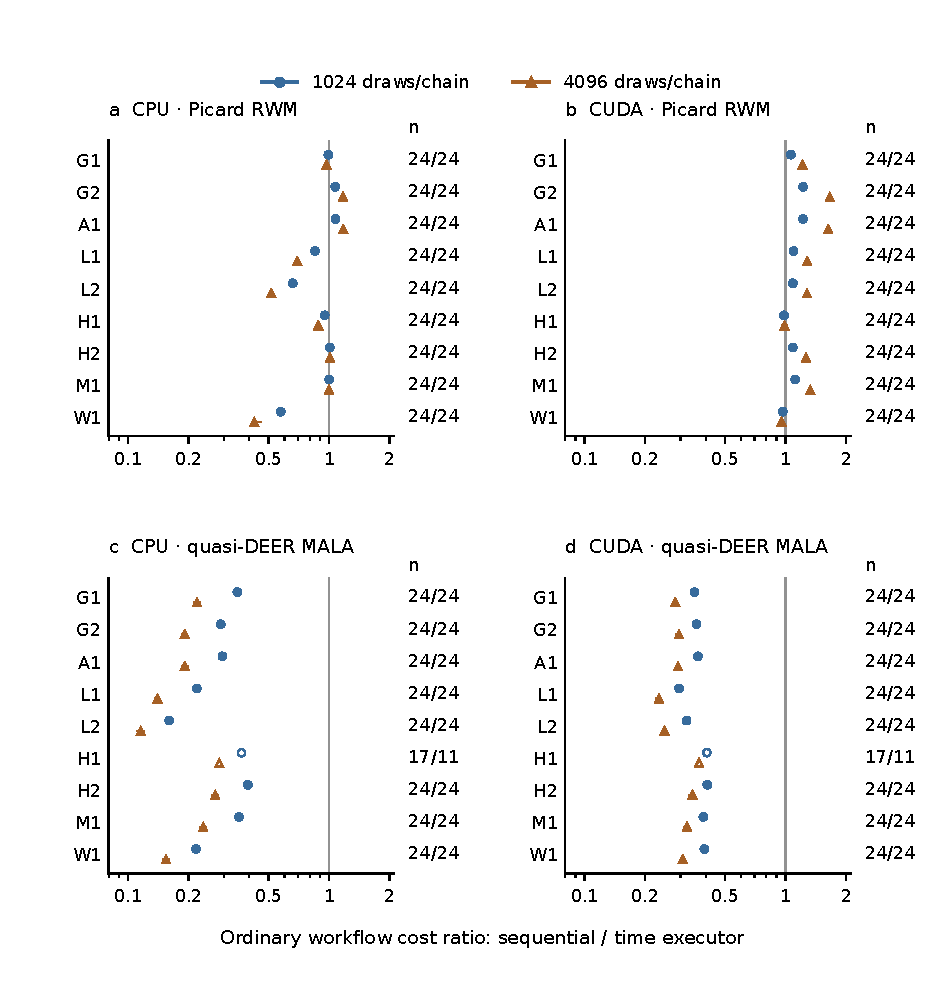
\includegraphics[width=\linewidth]{../../figures/compact-final-v1/ordinary-cost-overview.pdf}
\caption{普通批量推断的同核速度比。上排Picard的收益依赖设备，下排quasi-DEER均较慢。点为配对几何平均，横线为逐点95\% BCa区间；圆点/三角对应每链1024/4096步。右侧为两预算配对数，空心点表示少于20对而未计算区间。}\label{fig:compact-cost}
\end{figure}

固定费用确实影响速度比，但不足以解释所有减速。W1的CPU顺序RWM平均4.94秒中，采样/丢弃及转换为2.52秒，启动、导入、间隙与退出的余量为1.81秒，目标准备0.10秒，输出0.01秒，函数与R诊断0.50秒。约一半费用在采样段之外。CPU Picard的采样段则为9.29秒，quasi-DEER为66.44秒；因此它们在该案例的执行费用本身也更高。九工作流、216次长预算拟合的完整分段记录见补充材料A。

表\ref{tab:three-costs}用同四份W1输入并列三种计时，避免把缓存子集与全部24次重复混为一组。CPU RWM的准备后比值0.276，加入普通批量开销后为0.414，再加入研究核验后为0.592：共同费用把减速比推向1。本例CUDA Picard在三个边界下都接近1。该表只有四份输入，作为描述性对照；主实验的24次配对区间仍以图\ref{fig:compact-cost}为准。
\begin{table}[htbp]\centering\small
\begin{tabular}{lrrr}\toprule
同核配对 & 准备后内核 & 普通批量推断 & 含核验研究运行\\\midrule
CPU Picard & 0.276 & 0.414 & 0.592\\
CPU quasi-DEER & 0.113 & 0.152 & 0.233\\
CUDA Picard & 0.996 & 0.966 & 0.976\\
CUDA quasi-DEER & 0.262 & 0.307 & 0.401\\
\bottomrule\end{tabular}
\caption{W1每链4096步的三种速度比（顺序/时间执行）。各列均使用原重复0、8、16、23，配对几何平均；缓存每输入四次调用先取其均值。本表不计算四重复区间。}\label{tab:three-costs}
\end{table}


\subsection{每轮推进量与重复工作解释窗口效应}
并行窗口同时提供计算机会和重复工作。设准备后顺序每步费用为$c_{\rm seq}$，时间执行器每轮平均确认$p$个转移、完整轮次平均费用为$C_{\rm round}(W)$，则稳态记账关系为
\begin{equation}\label{eq:cost-model}
S\approx\frac{p\,c_{\rm seq}}{C_{\rm round}(W)},\qquad
\text{等长quasi-DEER窗口中 }p=W/\overline K.
\end{equation}
这里$C_{\rm round}$包含映射、JVP、扫描、控制与同步，而非只计一次批量密度求值；准备、尾部窗口和测量扰动另列。这是费用关系，不是已经拟合和验证的跨模型预测器。

既有Mac机制对照中，G1四链Picard把窗口16增至64，每轮确认数的组中位数仍约5.57；前向映射调用由5.50增至20.88次/输出转移，速度比从0.402降至0.170。G2单链quasi-DEER的平均窗口轮数从11增至22.25，速度比从0.051降至0.027。窗口扩大增加的工作超过了确认推进的改善。Windows机制对照亦记录步长、窗口及链数的影响，但每模型只有两份机制输入；分段探针尚未唯一分离扫描、JVP和主机控制的贡献。

\subsection{核选择改变误差，配对执行主要改变时间}
G2和A1在4096步下表现出明显核差异：RWM标准化首参数函数在24/24次拟合中有$\hat R>1.01$，MALA均未超过该阈值，两设备一致。这两个目标已经白化，差异反映给定维度与配置下的转移性质。图\ref{fig:error-cost}显示，同核执行通常沿时间方向改变位置，核与参数化则可以改变函数误差。

这种优势并不普遍。L1长预算的MALA有2/24份拟合探索不足，RWM在该函数的平均平方误差更低。原重复21中，一条MALA链在4096个保留转移只接受202次；两执行的接受记录相同，$q_1$最大路径差约$4.5\times10^{-11}$，但分位数处的并列值随浮点运算次序改变，tail ESS分别为4.81与31.88。直接二进制重算定位到5\%分位数的指示序列；两者$\hat R$都超过1.30。ESS差异在这里反映对大量重复状态的数值敏感性，保留两套原结果可避免把它误读为统计信息增加。复核与仅用于解释的舍入敏感性检查见补充材料A。
\begin{figure}[htbp]\centering
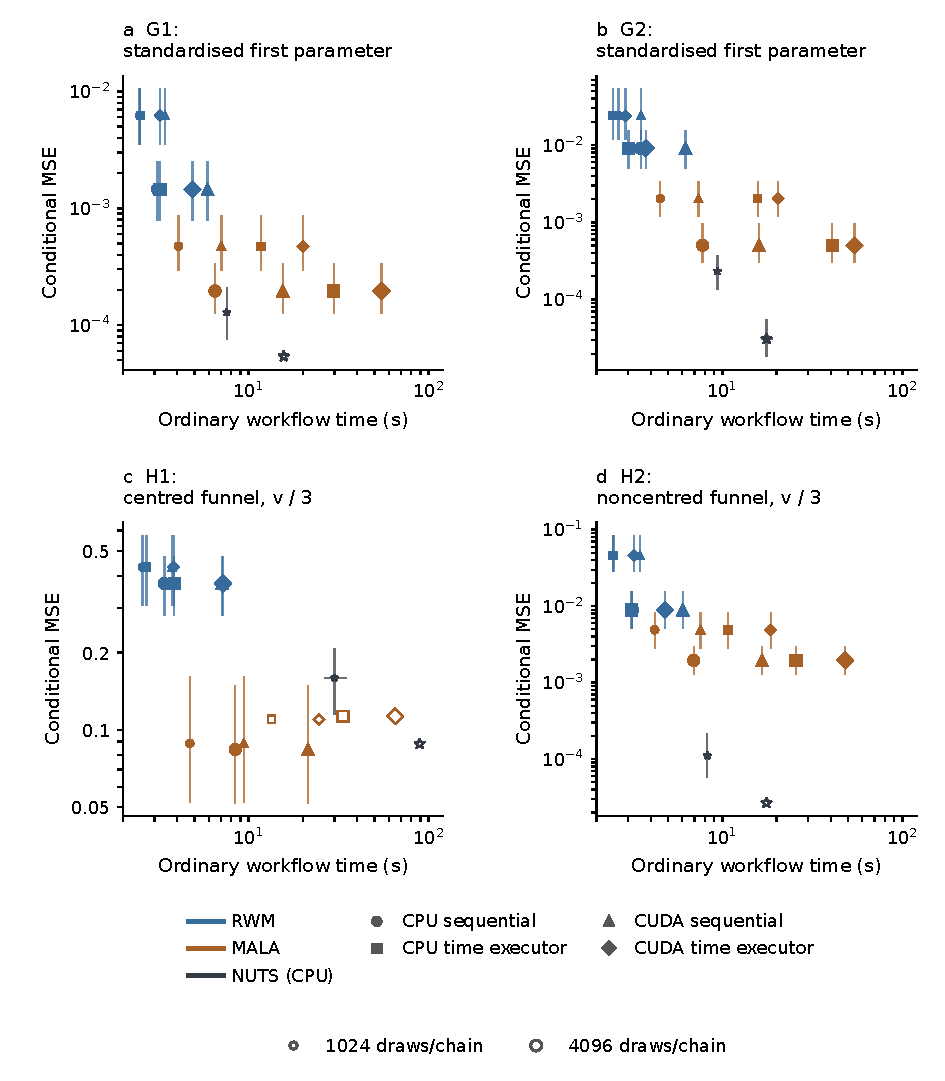
\includegraphics[width=\linewidth]{../../figures/manuscript-v5/error-cost/error-cost-overview.pdf}
\caption{四个代表函数在已测预算上的误差--成本。颜色表示RWM、MALA或NUTS，形状区分设备与执行方式，点大小区分1024/4096步；横纵线为逐点95\% BCa区间，空心点为区间未定。G1/G2及漏斗两种坐标用于事后机制解释，九目标36函数的全部结果见补充材料B。}\label{fig:error-cost}
\end{figure}

探索困难主要集中在中心化漏斗：其1500个有效拟合--函数诊断中1387个有限$\hat R>1.01$，水井的3024个函数诊断中为56个。所有函数级记录见补充材料A、B。

CPU NUTS的4096步工作流有105/216项未返回完整四链输出，1024步216项均完成。有限定位在部分G2/A1条件下发现完整采样保存后的旧诊断内存故障，旁路该诊断后完成；六个选定历史失败输入在新仪器化工作流中未复现。原105项仍为未分类运行失败，长预算部分目标的NUTS误差仅由4--9份有效拟合估计，G2/A1/W1则各有24份；该基线的成功条件结果和失败成本共同呈现（补充材料A）。

\subsection{水井应用：最快调用与较小误差的取舍}
W1使用3020份距离与换井观测，模型为$\Pr(y_i=1)=\sigma(\alpha+\beta d_i/100)$，$\alpha,\beta$使用平坦先验。我们估计回归系数及0米/100米的预测概率。数据中两个不同距离均有相反结局，足以证明这个二维后验可正规化；对应观测和证明见补充材料A。

数值区间参考给出$\E[\beta]\approx-0.623$，$\E[p(0)]\approx0.647$、$\E[p(100)]\approx0.496$。独立MCMC参考的95\%等尾区间分别为$[-0.811,-0.430]$、$[0.620,0.673]$和$[0.465,0.526]$；均值区间与分位数的有限样本误差分别解释。

CPU顺序RWM是本例费用最低的工作流（4.9秒）。NUTS用约2.4倍时间，将$\alpha$的参考平方误差降至约七分之一；CPU顺序MALA处于两者之间（表\ref{tab:wells-v5}）。同核时间并行增加耗时，而函数误差在表的显示精度下相同，因此合并列示。W1连续函数的参考区间半宽均不超过$10^{-8}$，传播到既有配对平方损失差后，其数值点排序不变；统计区间的抽样波动另见补充材料A。
\begin{table}[htbp]\centering\small
\begin{tabular}{lrrrr}\toprule
核 & CPU顺序 & CPU时间执行 & CUDA顺序 & CUDA时间执行\\\midrule
RWM & 4.94 & 11.59 & 5.73 & 6.01\\
MALA & 10.58 & 68.85 & 13.99 & 45.51\\
NUTS & 11.62 & --- & --- & ---\\\bottomrule
\end{tabular}
\par\medskip
\begin{tabular}{lrr}\toprule
核 & $\alpha$参考平方误差（$10^{-6}$） & $\beta$参考平方误差（$10^{-6}$）\\\midrule
RWM & 2.06 [1.16, 3.40] & 4.91 [2.72, 7.94]\\
MALA & 0.58 [0.39, 0.89] & 1.11 [0.68, 2.00]\\
NUTS & 0.28 [0.14, 0.51] & 0.52 [0.32, 0.84]\\\bottomrule
\end{tabular}
\caption{W1每链4096步的普通批量推断时间均值（秒，上表）和参考平方误差（下表）。每工作流24次四链重复；同核误差在显示精度下相同，合并列示。方括号为条件95\% BCa区间，参考区间的影响另见补充材料A。}\label{tab:wells-v5}
\end{table}


\subsection{三个容易误读的“好结果”}
\paragraph{执行快可以来自一条不移动的链。}
首轮Windows的A1/RWM配置全部拒绝提议，CUDA Picard的准备后执行却约快4.09倍。重复初值让执行器一次确认整个窗口，减少了求解工作，同时没有产生后验探索。这一历史反例与主实验使用不同配置，完整身份见补充材料A。

\paragraph{合并峰权重可以由初值维持。}
M1的412份有效拟合中，411份保存路径未穿越零点，但合并正侧比例恰为$1/2$。两条链从负侧、两条从正侧出发，等长合并自然维持这一比例。唯一穿越例为一次短预算NUTS拟合的一条链（补充材料A）。已知模式权重时可研究分层估计；这里的零符号误差本身并未说明单链跨峰充分。

\paragraph{极小绝对误差可以掩盖相对误差。}
L2的符号事件由两套重要性参考估计约为$1.6\times10^{-9}$与$1.8\times10^{-9}$，414份有效拟合的经验频率全为零。W1事件$\beta>0$的向外舍入数值区间为$[4.7671124,4.7673026]\times10^{-11}$，其经验频率同样全零。两者相对参考误差均为100\%，绝对平方误差却极小。即使把保存状态假想为独立后验抽样，期望命中也只有约0.0065和0.00021次；实际轨迹还相关。因此当前样本频率无法提供有用的事件相对精度。两套L2参考的近似MCSE及重要性权重稳定性、W1数值余项和理想独立参照见补充材料A。

\section{讨论与结论}
\subsection{对实际使用的含义}
本研究发现三种不同费用效应：CUDA提高了所测Picard工作流的多数加速点估计；quasi-DEER的重复工作在全部指定组中超过执行收益；启动与核验等共有费用把速度比推向1。W1进一步给出误差与时间的取舍，L1则说明合理移动距离调参也可能留下偶发停滞。对廉价目标，顺序执行是值得先测量的对照；选择时间执行器时，应在同实际输入上检查路径，再结合完整调用费用和具体函数诊断。

这些结果与原文报告的加速处于不同计算条件。Picard在Apple M3上对由时滞微分方程定义的昂贵黑箱似然报告约2.52倍墙钟收益\cite{grazzi}；本研究多数目标的密度计算更廉价。扩大数据量或引入昂贵似然可研究单次求值与批处理吞吐的交叉条件，但现有记录只支持指定成本结构下的比较。式\eqref{eq:cost-model}提供测量思路，尚未给出这种交叉点的预测。

使用者可以分别检查三个问题：每轮确认多少步、为推进这些步重复了多少工作；所关心函数的误差与原尺度含义；单链是否离开初值并探索模式或尾部。窗口、接受率和并列值都影响这些判断。共享轨迹的执行比较与不同核的推断比较放在不同层次，才能解释速度变化究竟来自计算顺序还是统计机制。

\subsection{适用范围与待解决问题}
本文评价固定维度连续目标、指定CPU/CUDA及含Python轮次控制的两类适配实现。窗口32未按各目标优化，代码融合、设备控制或昂贵目标可能给出不同结果；本文也没有复现上游最优加速配置。Stan入口目前仅支持CPU顺序RWM/MALA，GPU NUTS和更广的多链基线尚未实测。合法的支持集外$-\infty$密度仍与数值失败统一处理，限制了部分有界支持目标。

主实验设计是在早期大网格启动后受资源约束调整的，具有独立实验身份，但并非完全事前预注册。速度与误差条件于规定数值标准和有效集合，H1失败与部分NUTS小样本限制总体排名。所选函数、两档预算与24次重复支持固定预算比较，不能精确识别连续的达标时间或一般后验误差保证。原105项失败的原因仍需扩大定位；关闭旧诊断的全目标NUTS重跑应作为新协议，保留原始失败及成本。

\subsection{结论}
ParallelBayes使指定MCMC递推的不同执行方式能够共享实际随机数组并接受独立检查。所测Picard的收益依赖设备，quasi-DEER在当前配置下较慢；两者的统计价值仍取决于核、初始化和推断函数。分段费用与重复状态的分析将执行成本、浮点核验和探索诊断联系起来，为后续昂贵目标及配置优化提供可重复的比较基础。

\section*{代码与数据可得性}
源码采用MIT许可，论文构建输入和复现指南见\href{https://github.com/AlchemistXC/ParallelBayes}{ParallelBayes仓库}及本版材料清单。历史CPU原始证据已在\href{https://github.com/AlchemistXC/ParallelBayes/releases/tag/cpu-review-v1}{cpu-review-v1 Release}公开；Windows主实验、有限NUTS定位与新增参考的完整原件仍需作者提供受控访问，当前源码和TeX包可重建图文，完整数值复现还需这些原件。补充材料A给出版本与分析身份，仓库\texttt{docs/REVIEWER-ACCESS.md}说明访问组件；公开归档范围、长期标识及审稿访问方式由作者在投稿前确定。

生成式工具用于辅助代码、分析组织、图表和中文表述。最终科学判断与稿件责任属于作者。
\begin{thebibliography}{99}\fontsize{10pt}{12pt}\selectfont\setlength{\itemsep}{2pt}
\bibitem{zoltowski} Zoltowski D.M., Wu S., Gonzalez X., et al. \href{https://proceedings.nips.cc/paper_files/paper/2025/hash/202886ee1c9ca735cb5bff3a00a69883-Abstract-Conference.html}{Parallelizing MCMC Across the Sequence Length}. Advances in Neural Information Processing Systems, 2025, 38.
\bibitem{grazzi} Grazzi S., Zanella G. \href{https://doi.org/10.1093/biomet/asag022}{Parallel computations for Metropolis Markov chains with Picard maps}. Biometrika, 2026, 113(2): asag022.
\bibitem{comparemcmcs} NIMBLE development team. \href{https://github.com/nimble-dev/compareMCMCs}{compareMCMCs: Tools for comparing MCMC efficiency from NIMBLE and other engines}. 软件作者仓库，访问于2026年10月3日。
\bibitem{pplbench} Kulkarni S., Shah K.D., Arora N., et al. \href{https://arxiv.org/abs/2010.08886v1}{PPL Bench: Evaluation Framework For Probabilistic Programming Languages}. arXiv:2010.08886v1, 2020. 软件来源：\url{https://github.com/facebookresearch/pplbench}。
\bibitem{posteriordb} Magnusson M., Torgander J., Bürkner P.-C., Zhang L., Carpenter B., Vehtari A. \href{https://proceedings.mlr.press/v258/magnusson25a.html}{posteriordb: Testing, Benchmarking and Developing Bayesian Inference Algorithms}. Proceedings of Machine Learning Research, 2025, 258:1198--1206.
\bibitem{parallelmcmc} Senne R. and contributors. \href{https://github.com/rsenne/ParallelMCMC.jl/tree/7be9c866c8be03ad994a5e7f0486ec3290088813}{ParallelMCMC.jl}. 软件仓库，提交7be9c86，访问于2026年10月6日。
\bibitem{bayesforge} Sosa S. \href{https://cran.r-universe.dev/BayesForge/doc/manual.html}{BayesForge: Bayesian Inference using numpyro and XLA}. R包0.0.1参考手册，访问于2026年10月6日。
\bibitem{gonzalez} Gonzalez X., Warrington A., Smith J.T.H., Linderman S.W. \href{https://arxiv.org/abs/2407.19115v3}{Towards Scalable and Stable Parallelization of Nonlinear RNNs}. arXiv:2407.19115v3, 2025（初版2024）.
\bibitem{stan} Carpenter B., Gelman A., Hoffman M.D., et al. \href{https://doi.org/10.18637/jss.v076.i01}{Stan: A Probabilistic Programming Language}. Journal of Statistical Software, 2017, 76(1): 1--32.
\bibitem{bridgestan} Roualdes E.A., Ward B., Carpenter B., Seyboldt A., Axen S.D. \href{https://doi.org/10.21105/joss.05236}{BridgeStan: Efficient in-memory access to the methods of a Stan model}. Journal of Open Source Software, 2023, 8(87):5236.
\bibitem{blackjax} Cabezas A., Corenflos A., Lao J., Louf R., et al. \href{https://arxiv.org/abs/2402.10797}{BlackJAX: Composable Bayesian inference in JAX}. arXiv:2402.10797, 2024.
\bibitem{pyro} Bingham E., Chen J.P., Jankowiak M., et al. \href{https://jmlr.org/papers/v20/18-403.html}{Pyro: Deep Universal Probabilistic Programming}. Journal of Machine Learning Research, 2019, 20(28):1--6.
\bibitem{posterior} Stan development team. \href{https://mc-stan.org/posterior/reference/rhat.html}{posterior: Rhat, bulk ESS and tail ESS documentation}. 软件文档，版本1.7.0。
\bibitem{vehtari} Vehtari A., Gelman A., Simpson D., Carpenter B., Bürkner P.-C. \href{https://doi.org/10.1214/20-BA1221}{Rank-Normalization, Folding, and Localization: An Improved R-hat for Assessing Convergence of MCMC}. Bayesian Analysis, 2021, 16(2):667--718.
\bibitem{modrak} Modrák M., Moon A.H., Kim S., et al. \href{https://doi.org/10.1214/23-BA1404}{Simulation-Based Calibration Checking for Bayesian Computation: The Choice of Test Quantities Shapes Sensitivity}. Bayesian Analysis, 2025, 20(2):461--488. DOI:10.1214/23-BA1404.
\end{thebibliography}

\end{document}
